%--------------------------------------
% Create title frame
\titleframe

%--------------------------------------
% Table of contents
\begin{frame}[allowframebreaks]{Overview}
  \setbeamertemplate{section in toc}[sections numbered]
  \tableofcontents%[hideallsubsections]
\end{frame}


% What will we learn slide
\begin{frame}{What will we learn today?}
    \begin{itemize}
        \item The power transformer
        \item The next part of power flow analysis: how to include transformers and transformers with tap changers
    \end{itemize}
    You will be able to do exercises 6.2, 6.3, 6.4 from Ned Mohan's book.
\end{frame}



\section{The Transformer}
% Three-phase system slide
\begin{frame}{Basic model of a transformer}
A (single phase) transformer is made of two magnetically coupled \alert{coils} or \alert{windings}.
An ideal transformer is a two-port represented as 
\begin{columns}
    \begin{column}{0.45\textwidth}
        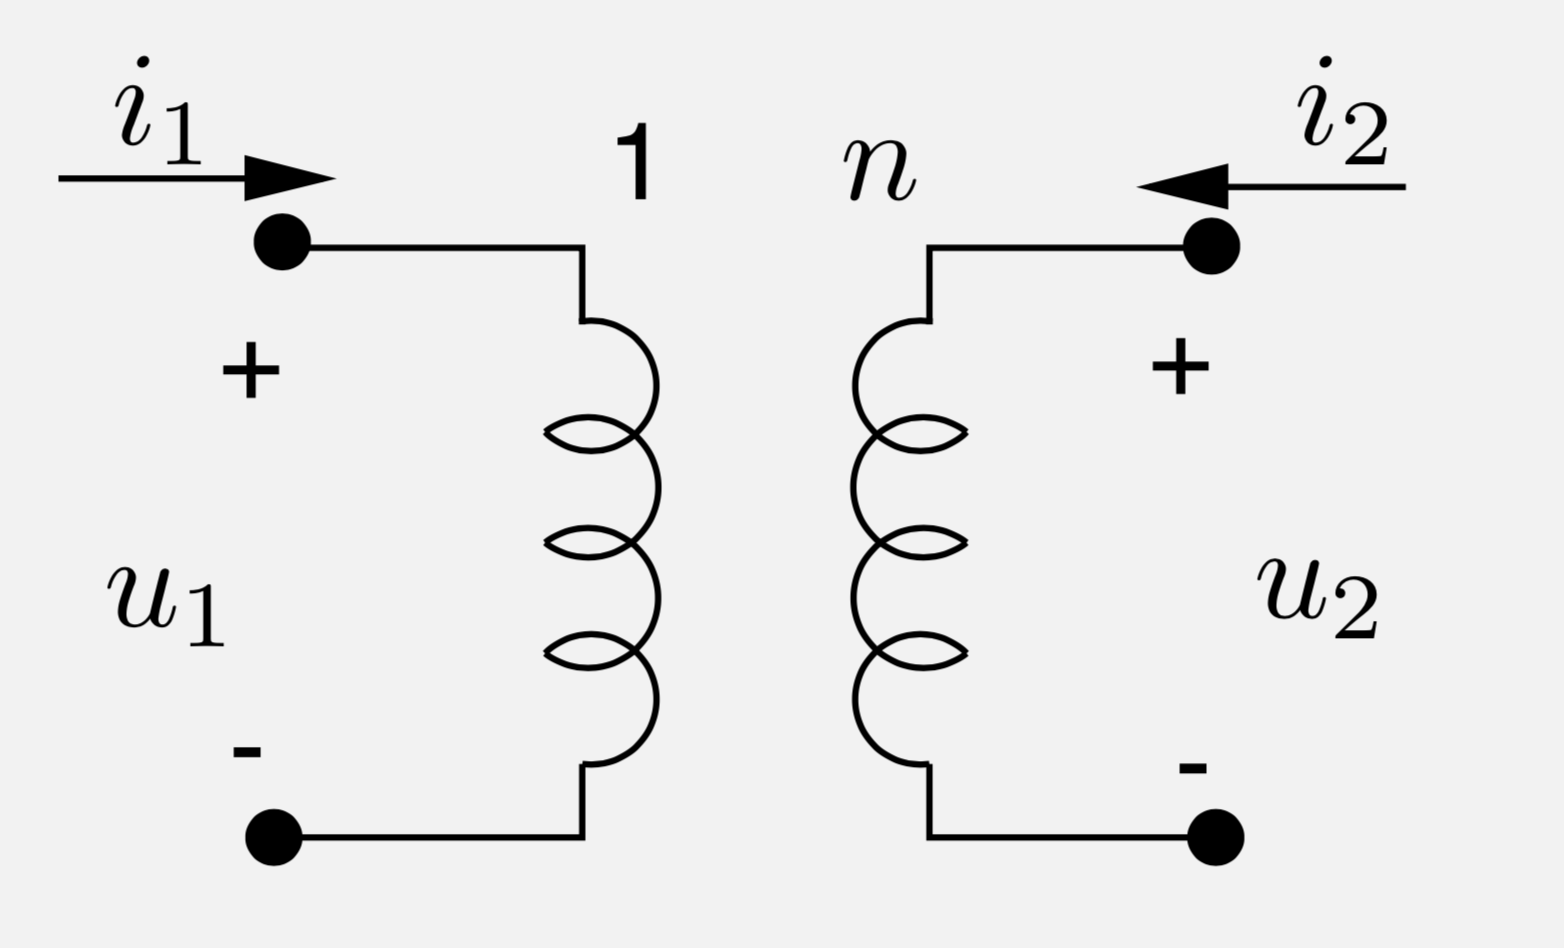
\includegraphics[width=\textwidth]{images/ideal_transformer.png}
    \end{column}
    \begin{column}{0.35\textwidth}
        with
        \begin{align*}
        u_2  &= n u_1 \\
        i_2  &= -\frac{1}{n}i_1
        \end{align*}
    \end{column}
\end{columns}
\end{frame}

\begin{frame}{Usages}
In power systems, transformers are mainly used to transmit power over long distances by changing the voltage level, 
thus decreasing the current for a given power level. The voltage level of a synchronous generator is around 20kV.

Voltage is changed around five times between generation and load.

It is also used to 
\begin{itemize}
    \item \alert{measure} currents and voltages, 
    \item electrically \alert{isolate} parts of a circuit (not the auto-transformer we will see), 
    \item and \alert{match} impedances.
\end{itemize}
\end{frame}

\begin{frame}{How does a transformer work?}
\begin{center}
    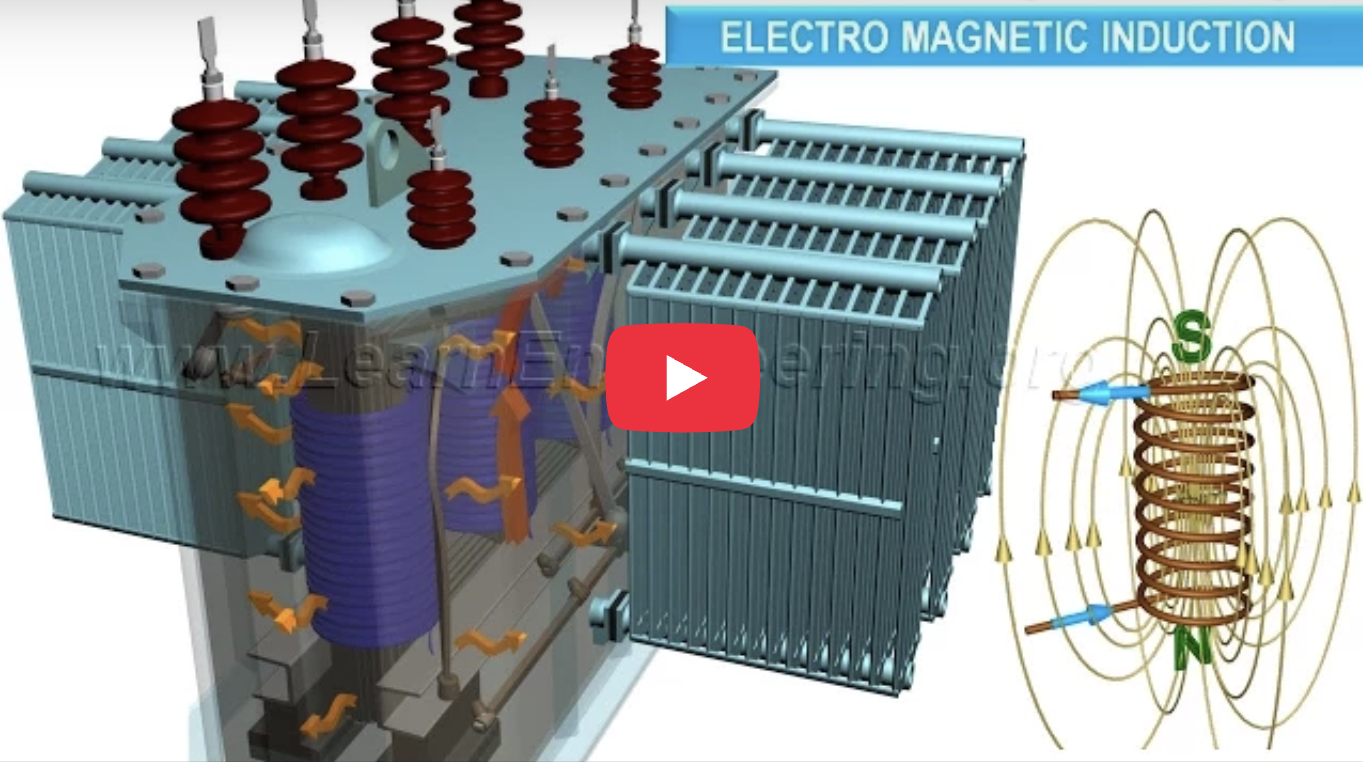
\includegraphics[width=0.6\textwidth]{images/how_a_tfo_works.png}\\
    \href{https://youtu.be/vh_aCAHThTQ}{\underline{Link to the video}}
\end{center}
\end{frame}

\begin{frame}[allowframebreaks]{Non-ideal model}

\begin{center}
   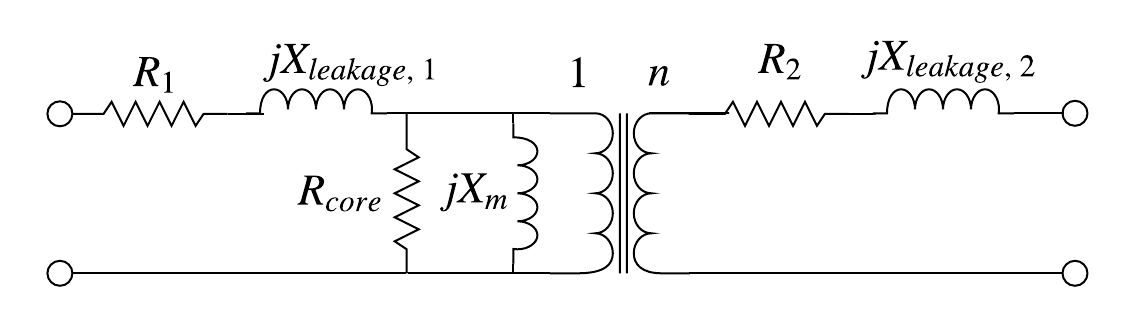
\includegraphics[width=0.9\textwidth]{images/non-ideal-transformer.png}
\end{center}
The ideal model is complemented by elements 
\begin{itemize}
    \item $X_m$ that models the magnetizing inductance
    \item $X_{leakage, i}$ that models the flux not captured by the core on side $i$
    \item $R_{core}$ that models eddy current and hysteresis losses, i.e., losses in the iron core
    \item $R_{1}$ and $R_{2}$ that model (coil) copper losses
\end{itemize}

Parameters are either given in the datasheet or obtained by open-circuit and short-circuit tests.

The core is ususally \alert{laminated}  to decrease losses.
\end{frame}

\begin{frame}{Simplification}

\begin{columns}
\begin{column}{0.45\textwidth}
    The excitation current, the sum of the currents in $R_{core}$ and $X_m$, is often neglected, 
    leading to a simpler non-ideal model, and the series impedances can be transferred from one side to the other, 
    with $$Z_p = R_1 + jX_{leakage, 1}$$ and $$Z_s = R_2 + jX_{leakage, 2}$$
\end{column}
\begin{column}{0.5\textwidth}
    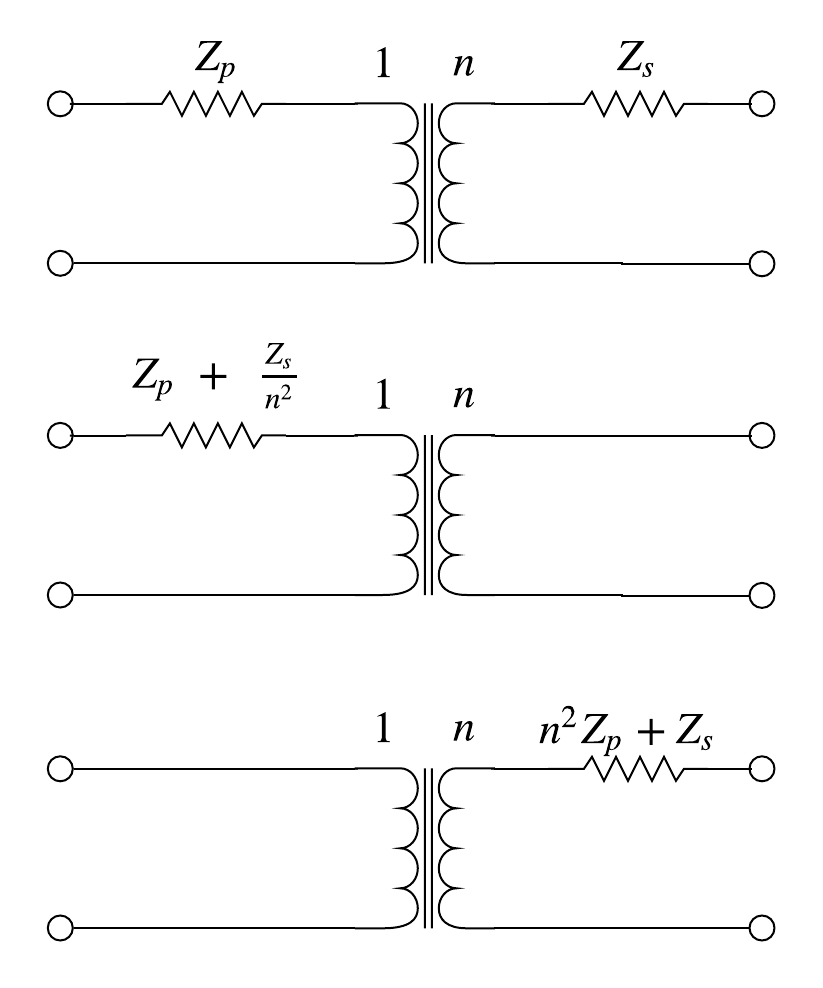
\includegraphics[width=0.8\textwidth]{images/non-ideal-transformer-2.png}
\end{column}
\end{columns}
\end{frame}

\begin{frame}[allowframebreaks]{Per unit representation}
Let's consider the rated voltages and currents on both sides of the (ideal) transformer as base values. As
$$V_{s, base} = n V_{p, base} $$ and $$ I_{p, base} = n I_{s, base},$$
the \alert{MVA base is the same on both sides}, and thus
$$Z_{s, base} = n^2 Z_{p, base}$$


\begin{columns}
    \begin{column}{0.55\textwidth}
        Hence, \alert{in per unit, the transformer can be replaced by a single impedance}
        $$Z_{tr} = \frac{Z_{p}}{Z_{p, base}}+\frac{Z_{s}}{Z_{s, base}}.$$
    \end{column}
    \begin{column}{0.45\textwidth}
        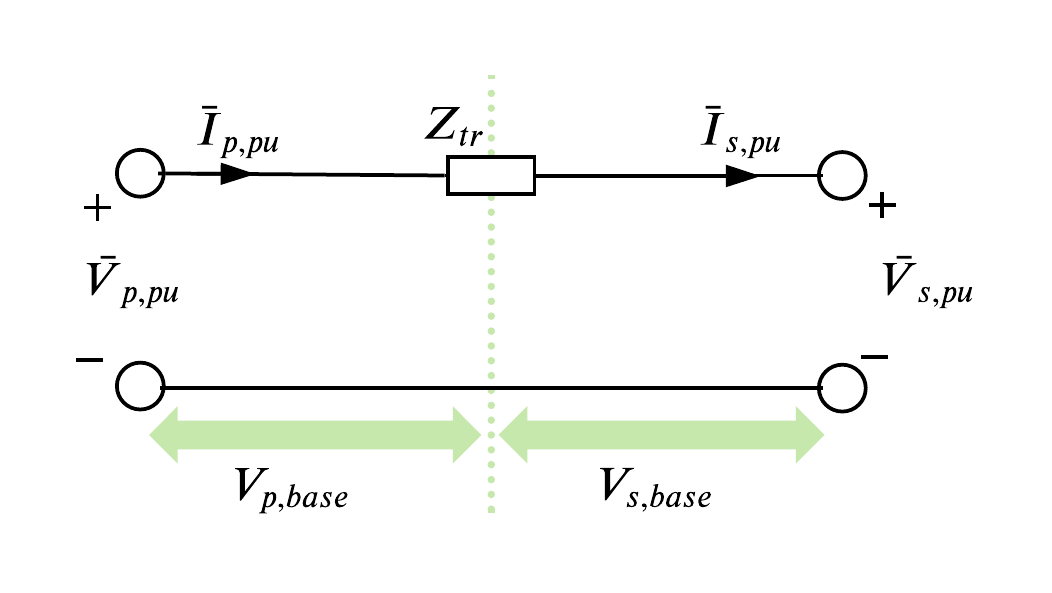
\includegraphics[width=\textwidth]{images/tfo-pu.png}
    \end{column}
\end{columns}

Thus we have also that 
\begin{align*}
    Z_{tr} &= \frac{Z_{p}+ Z_s/n^2}{Z_{p, base}} \\
     &= \frac{n^2 Z_{p} + Z_s}{Z_{s, base}}
\end{align*}
i.e. \alert{the impedance is the same whether we see it from the primary or the secondary side, although the voltage bases differ}.

Also, if the three-phase transformer is \alert{wye-delta} connected, a \alert{30° phase shift} must be applied (more on this later).
\end{frame}


\begin{frame}[allowframebreaks]{Illustration of Per-Unit normalization}

This is Example 6.1 from the reference book. Consider the one-line diagram 
\begin{center}
    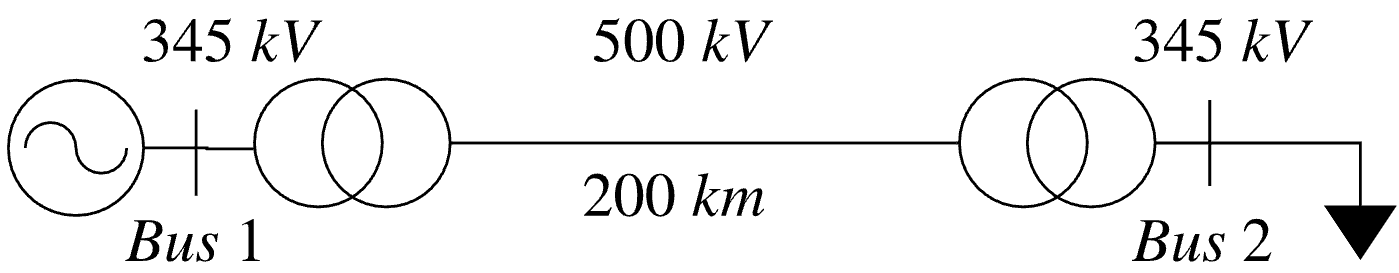
\includegraphics[width=0.6\textwidth]{images/example-6-1.png}
\end{center}
with 
\begin{itemize}
    \item a 200 km line with $R = 0.029 \Omega/km$, $X=0.326 \Omega/km$, neglected shunt impedances
    \item two transformers with a leakage reactance of $0.2 pu$ in the (500 kV, 1000 MVA) base, and losses neglected.
\end{itemize}
\alert{What is the equivalent model in a (345 kV, 100 MVA) base?}



\textbf{In the (500 kV, 1000 MVA) base:}
\begin{itemize}
    \item $Z_{line, pu} = 200 \times (0.029 + j 0.326) / (500^2/1000) = 0.0232 + j 0.2608 pu$
    \item hence, the total impedance between buses 1 and 2 is $$Z_{12} = 0.0232 + j 0.2608  + 2 * j 0.2pu =  0.0232 + j 0.6608 pu $$
\end{itemize}


\textbf{In the (345 kV, 100 MVA) base}
\begin{itemize}
    \item the pu value of the impedance is the same in the (\alert{500} kV, 1000 MVA) and (\alert{345} kV, 1000 MVA) bases! 
    \item Why? since we can transfer the impedance from one side of each transformer to the other, cf. a previous remark.
    \item if we now change the MVA base to 100 MVA, 
 $$Z_{12} = (0.0232 + j 0.6608)  \times (100/1000) pu =  0.00232 + j 0.06608 pu$$ since the base impedance is proportional to the inverse of the MVA base.
\end{itemize}
\end{frame}


\begin{frame}{Efficiency}

The efficiency expressed in \% is 
$$100 \times \frac{P_{output}}{P_{input}} = 100 \times \left(1 - \frac{P_{losses}}{P_{input}}\right) $$

Remarks: 
\begin{itemize}
    \item maximal when loaded such that copper losses = iron losses (cancel derivative of efficiency w.r.t current) 
    \item Around \alert{99.5 \%} in large power transformers at full load.
\end{itemize}
\end{frame}


\begin{frame}{Tap changers}

\begin{itemize}
\item Some transformers are equipped with a system allowing to change the $1:n$ ratio
\item The ability to change the tap under load is called load tap changer (LTC) or on-load tap changer (OLTC)
\item This is mainly used for voltage control
\item It is usually implemented using auto-transformers
\item We will see later on how to include this in the power flow analysis
\end{itemize}
\end{frame}

\begin{frame}{Tap changing transformers}
\begin{center}
    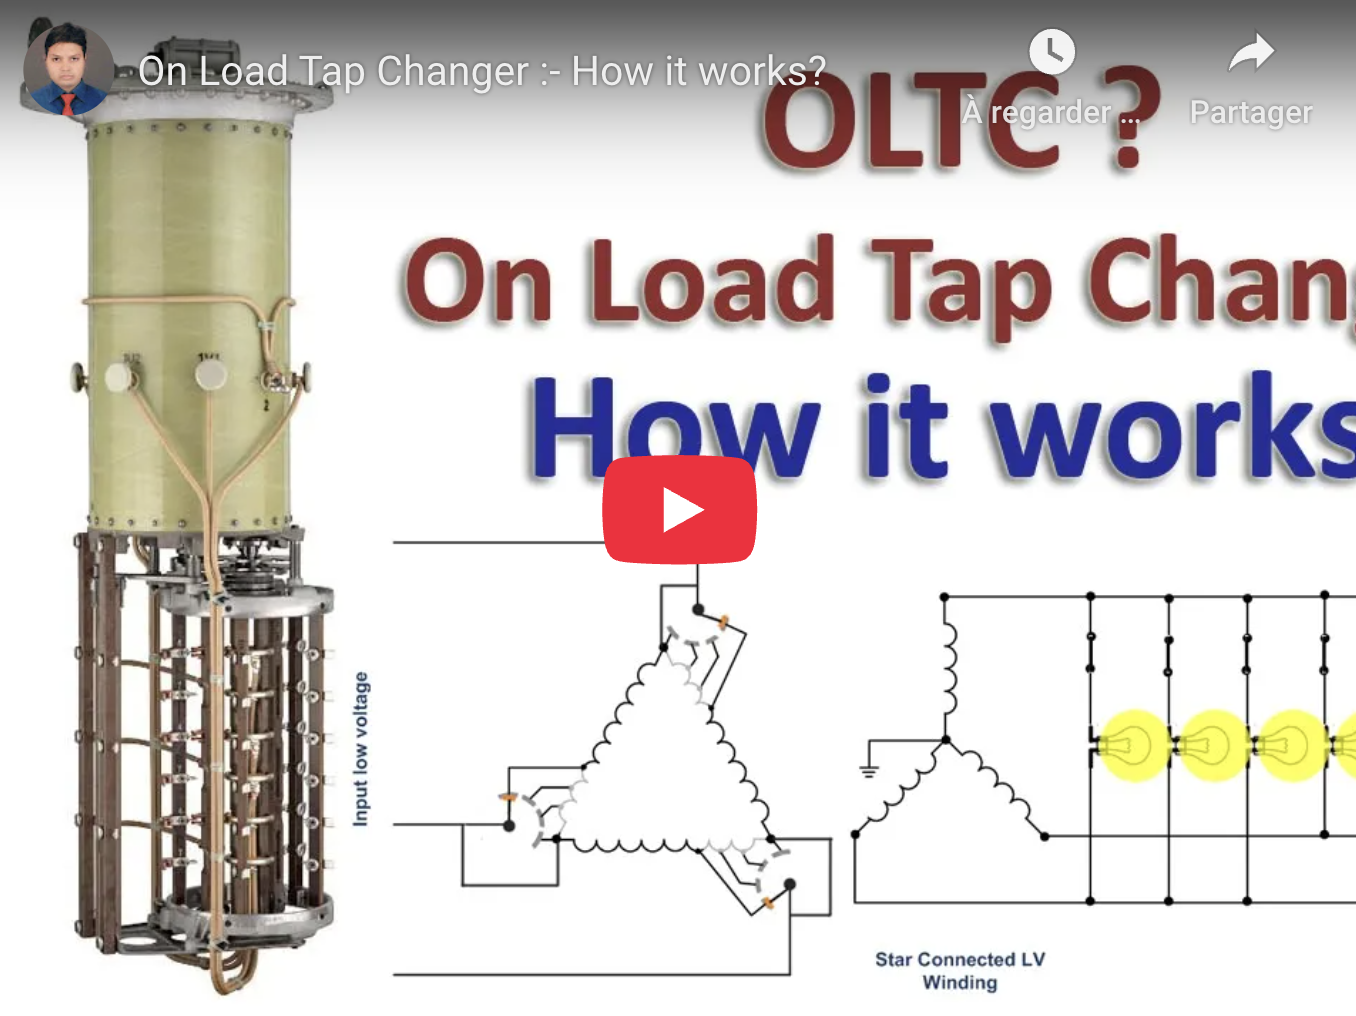
\includegraphics[width=0.5\textwidth]{images/OLTC.png}\\
    \href{https://www.youtube.com/embed/R_NxRDXOEFk}{\underline{Link to the video}}
\end{center}
\end{frame}

\begin{frame}{Auto-transformers}

The two windings (of the same phase) are connected in series, without galvanic insulation. 
They are commonly used when the ratio is limited.


\begin{columns}
    \begin{column}{0.45\textwidth}
Advantages: 
\begin{itemize}
\item Physically smaller
\item less costly (less copper)
\item higher efficiency
\item easy to implement tap changes
\item "solid" earth grounding
\end{itemize}
\end{column}
\begin{column}{0.45\textwidth}
Disadvantages:
\begin{itemize}
\item no electrical insulation
\item higher short circuit current
\item full voltage at secondary if it breaks (in case of a step down)
\end{itemize}
\end{column}
\end{columns}

\end{frame}

\begin{frame}{Phase shift in delta-star transformers}

The star part has $n$ times the number of turns of the delta part (primary side).


\begin{columns}
    \begin{column}{0.45\textwidth}
Let's reason on phase $a$,
\begin{itemize}
    \item Voltage $\bar{V}_{a,s}$ is on the same core as $\bar{V}_{AC,p} = \sqrt{3}\bar{V}_{a,p} \angle{-30^\circ}$ where $\bar{V}_{a,p}$ is the (virtual) phase-neutral voltage on the primary side.
    \item Since  $\bar{V}_{a,s} = n \bar{V}_{AC,p}$, $\bar{V}_{a,s} = n\sqrt{3} \bar{V}_{a,p} \angle{-30^\circ}$
\end{itemize}
    \end{column}
    \begin{column}{0.5\textwidth}
\begin{center}
    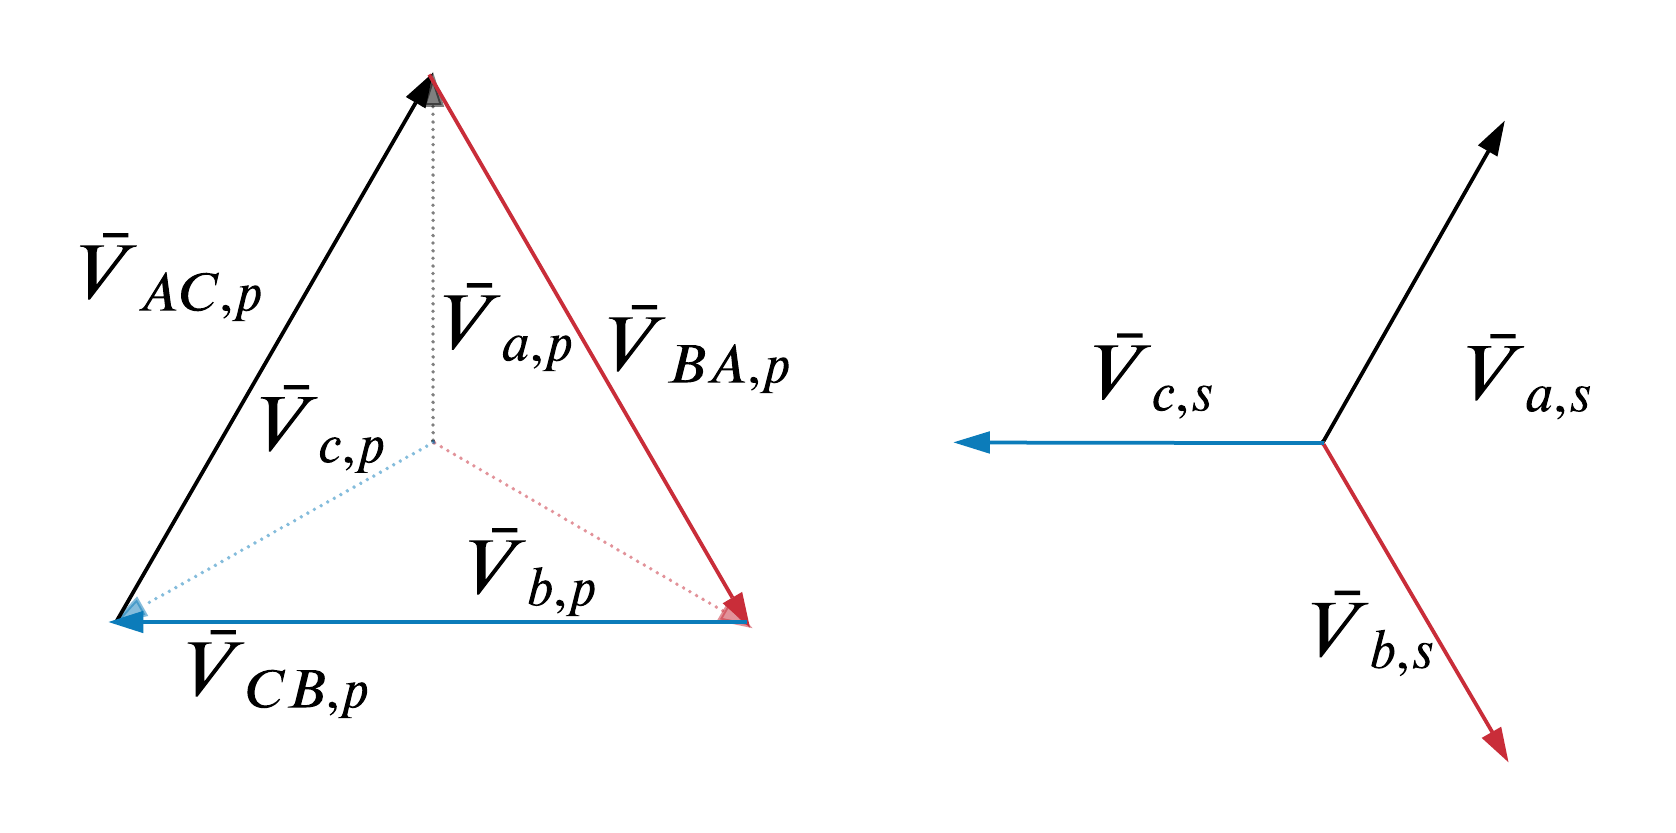
\includegraphics[width=\textwidth]{images/tfo-delta-star.png}\\
\end{center}
    \end{column}
\end{columns}

We \alert{gain a $\sqrt{3}$ factor} in the amplification, and a \alert{lagging phase shift of 30°}.

The same reasoning holds for phases $b$ and $c$.

\end{frame}

\begin{frame}[allowframebreaks]{Power flow regulation by phase shifting}

We have seen that active power flows are dictated by the voltage magnitudes but also the sine of the angle difference between buses: 

\begin{columns}
    \begin{column}{0.55\textwidth}
        \begin{center}
            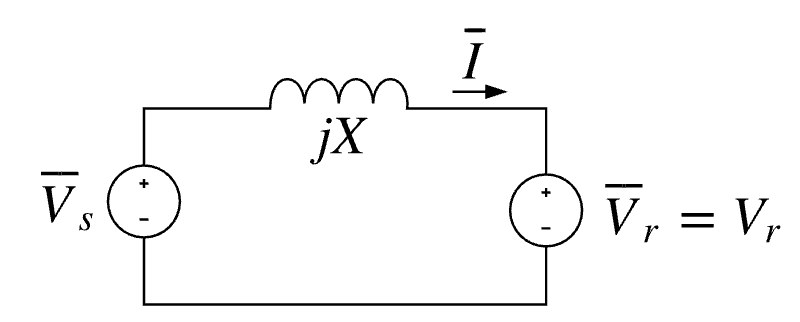
\includegraphics[width=\textwidth]{images/power-transfer_AC.png}\\
        \end{center}
    \end{column}
    \begin{column}{0.45\textwidth}
        \begin{align*}
        S_r &= \bar{V}_r\bar{I}^*  = V_r \left(\frac{V_s \angle -\delta - V_r}{-jX}\right) \\\\
            &= \frac{V_s V_r \sin \delta }{X} +j \frac{V_s V_r \cos \delta - V^2_r}{X} 
        \end{align*}
        $\delta$ is the angle between $\bar{V}_r$ and $\bar{V}_s$
    \end{column}
\end{columns}

If we have a device that can generate an adjustable phase shift, we can control the power flows.
This is the purpose of \alert{phase-shifting transformers}.

In practice phase shifting is achieved by "combining the signal with a fraction of itself shifted by 90°".
For the details of how it is implemented or modeled, see 
\begin{itemize}
    \item \href{https://en.wikipedia.org/wiki/Quadrature_booster}{\underline{Wikipedia}}
    \item Section 5.7. of the Weedy or ELEC0014.
    \item \href{https://eepublicdownloads.blob.core.windows.net/public-cdn-container/clean-documents/CIM_documents/Grid_Model_CIM/ENTSOE_CGMES_v2.4.14_28May2014_PSTmodelling.pdf}{\underline{ENTSO-E - Phase Shift Transformers Modelling, Version 1.0.0, May 2015}}
\end{itemize}

\end{frame}

\begin{frame}[allowframebreaks]{Example: phase shifting transformers on the borders of Belgium}

\begin{columns}
    \begin{column}{0.5\textwidth}
\begin{center}
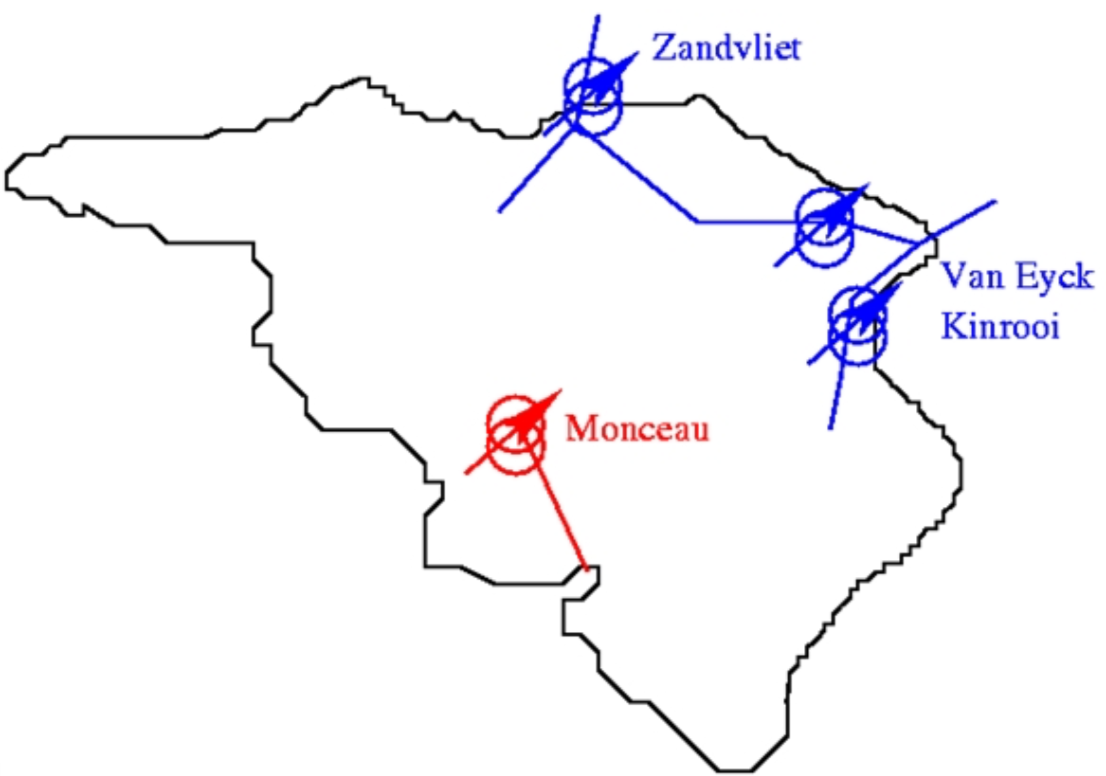
\includegraphics[width=\textwidth]{images/phase-shifters-be.png}        
\end{center}

    \end{column}
    \begin{column}{0.45\textwidth}
380/380 kV, in series with:
\begin{enumerate}
    \item line Zandvliet (B) - Borssele (NL) and Zandvliet (B) - Geertruidenberg (NL)
    \item line Meerhout (B) - Maasbracht (NL)
    \item line Gramme (B) - Maasbracht (NL)
    \begin{itemize}
        \item nominal power 3VN Imax = 1400 MVA
        \item phase shift adjustment: 35 positions, $+17/-17 \times 1.5°$ (at no load)
    \end{itemize}
\end{enumerate}

    \end{column}
\end{columns}
220/150 kV : 
\begin{itemize}
\item in series with the Chooz (F) - Monceau (B) line nominal power: 400 MVA
\item in-phase adjustment: 21 positions, $+10/-10 \times 1.5 \% $
\item quadrature adjustment: 21 positions, $+10/-10 \times 1.2°$
\end{itemize}

\end{frame}

\begin{frame}{Remarks}

In \alert{three-phase operation},
\begin{itemize}
\item either there are three separate single-phase transformers (easier to fix when there is a problem on a phase, more modular)
\item or a \alert{three-phase transformer}, that is a single core with three auto-transformers on it, cf. the video at the beginning of this presentation (cheaper, lighter core and less copper).
\end{itemize}
 
Some transformers called \alert{three-winding transformers} are equipped with a third winding (not to be confused with a three-phase transformer) that is used for auxiliary purposes (feeding auxiliary devices e.g., fans, providing reactive power support, ...).


\end{frame}

\section{Transformers in the power flow analysis}

\begin{frame}{Transformer without regulation}


A transformer, in the per-unit representation, can thus be represented 
\begin{itemize}
    \item as a two-port if the shunt admittance is considered
    \item as a simple series leakage impedance if the shunt admittance is neglected
\end{itemize}
 
It is a bit harder to model controllable taps for voltage and flow control.

\end{frame}

\begin{frame}[allowframebreaks]{Representing taps and phase shifts}


\begin{columns}
    \begin{column}{0.5\textwidth}
    Let $Y_l$ be the leakage admittance and $t$ be the off-nominal turns ratio:
    \begin{itemize}
        \item if $ 0 < t \leq 1$, this corresponds to a simple tap-changer
        \item if $ 0 < |t| \leq 1$ but is complex, then this is a phase-shifter ($\angle{t} < \pi/2$)
    \end{itemize}
    \end{column}
    \begin{column}{0.45\textwidth}
        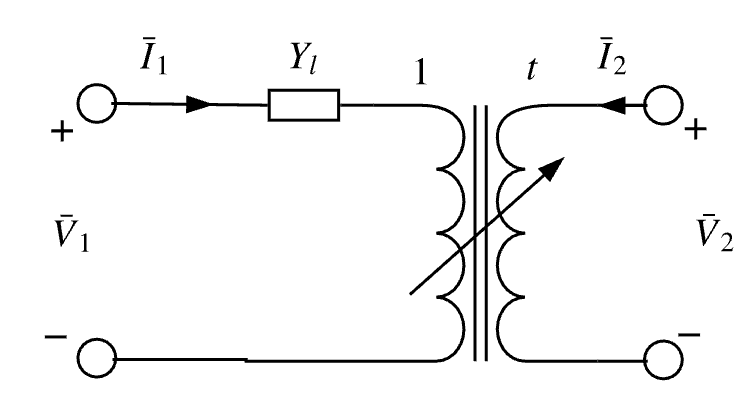
\includegraphics[width=\textwidth]{images/tap-shift-tfo.png}
    \end{column}
\end{columns}

We have 
$$\bar{I}_1 = \left(\bar{V}_1 - \frac{\bar{V}_2}{t}\right) Y_l$$
and since $\frac{\bar{V}_2}{t} \bar{I}_1^\star = -\bar{V}_2 \bar{I}_2^\star$ by energy conservation
$$\bar{I}_2 = - \frac{\bar{I}_1}{t^\star} = - \bar{V}_1 \frac{Y_l}{t^\star} + \bar{V}_2 \frac{Y_l}{|t|^2}$$

Thus tap and phase shift can be represented by the admittance matrix

$$\left[\begin{array}{c} \bar{I}_1 \\ \bar{I}_2\end{array}\right] 
 = \left[\begin{array}{c c} Y_l & -\frac{Y_l}{t} \\ -\frac{Y_l}{t^\star} & \frac{Y_l}{|t|^2} \end{array}\right]
 \left[\begin{array}{c} \bar{V}_1 \\ \bar{V}_2\end{array}\right]$$

 \newpage
\begin{itemize}
    \item if $ 0 < t \leq 1$, this can be represented as a $\pi$ two-port
    \item if $ 0 < |t| \leq 1$ but is complex, this is not the case
\end{itemize}

In the power flow analysis you must \alert{pay attention to this when constructing the system-wide admittance matrix.}
As an exercise, let's add a phase-shifting transformer to our 3-bus example.

\begin{itemize}
    \item \href{https://github.com/bcornelusse/ELEC0447-analysis-power-systems/blob/master/notebooks/PF_3_transformer_gen_limits_pandapower.ipynb}{\underline{Link to the example in PandaPower}}
    \item \href{https://github.com/bcornelusse/ELEC0447-analysis-power-systems/blob/master/notebooks/power_flow_3-bus-transformer_and_gen_limits_Newton-Raphson.py}{\underline{Link to the Newton-Raphson example}}
\end{itemize}

\end{frame}